%!TEX

% Тип документа
\documentclass[a4paper,12pt]{extarticle}

% Шрифты, кодировки, символьные таблицы, переносы
% \usepackage{cmap}
% \usepackage[T2A]{fontenc}
\usepackage[utf8]{inputenc}
\usepackage[russian]{babel}
% Это пакет -- хитрый пакет, он нужен но не нужен
\usepackage[mode=buildnew]{standalone}

\usepackage
	{
		% Дополнения Американского математического общества (AMS)
		amssymb,
		amsfonts,
		amsmath,
		amsthm,
		% Пакет для физических текстов
		physics,
		% misccorr,
		% 
		% Графики и рисунки
		wrapfig,
		graphicx,
		subcaption,
		float,
		tikz,
		tikz-3dplot,
		caption,
		csvsimple,
		color,
		booktabs,
		geometry,
		% 
		% Таблицы, списки
		makecell,
		multirow,
		indentfirst,
		%
		% Интегралы и прочие обозначения
		ulem,
		esint,
		esdiff,
		% 
		% Колонтитулы
		fancyhdr,
	}  
\usepackage{pgfplots,pgfplotstable,booktabs,colortbl}
\usepackage{xcolor}
\usepackage{hyperref}
\usepackage{gensymb}
\usepackage{textcomp}
\usepackage{qrcode}
\usepackage{appendix}
\usepackage[e]{esvect} % рисует нормальные вектора

\usepackage{mathtools}
\mathtoolsset{showonlyrefs=true}
 % Цвета для гиперссылок
\definecolor{linkcolor}{HTML}{000000} % цвет ссылок
\definecolor{urlcolor}{HTML}{799B03} % цвет гиперссылок
 
\hypersetup{pdfstartview=FitH,
			linkcolor=linkcolor,
			citecolor=linkcolor,
			urlcolor=urlcolor, 
			colorlinks=true}
\hypersetup{pageanchor=false}
% Увеличенный межстрочный интервал, французские пробелы
\linespread{1.3} 
\frenchspacing 

 
% \usetikzlibrary
% 	{
% 		decorations.pathreplacing,
% 		decorations.pathmorphing,
% 		patterns,
% 		calc,
% 		scopes,
% 		arrows,
% 		fadings,
% 		through,
% 		shapes.misc,
% 		arrows.meta,
% 		3d,
% 		quotes,
% 		angles,
% 		babel
% 	}
% Среднее <#1>
\newcommand{\mean}[1]{\langle#1\rangle}
% const прямым шрифтом
\newcommand\ct[1]{\text{\rmfamily\upshape #1}}
\newcommand*{\const}{\ct{const}}
\usepackage{array}
\usepackage{pstool}

\geometry		
	{
		left			=	2.5cm,
		right 			=	1.5cm,
		top 			=	2cm,
		bottom 			=	2cm,
		bindingoffset	=	0cm
	}

%%%%%%%%%%%%%%%%%%%%%%%%%%%%%%%%%%%%%%%%%%%%%%%%%%%%%%%%%%%%%%%%%%%%%%%%%%%%%%%
	%применим колонтитул к стилю страницы
\pagestyle{fancy} 
	%очистим "шапку" страницы
% \fancyhead{} 
	%слева сверху на четных и справа на нечетных
\fancyhead[R]{}%\labauthors 
	%справа сверху на четных и слева на нечетных
% \fancyhead[L]{Отчёт по лабораторной работе №\labnumber}
\fancyhead[L]{\labtheme} 
	%очистим "подвал" страницы
% \fancyfoot{} 
	% номер страницы в нижнем колинтуле в центре
\fancyfoot[C]{\thepage} 

%%%%%%%%%%%%%%%%%%%%%%%%%%%%%%%%%%%%%%%%%%%%%%%%%%%%%%%%%%%%%%%%%%%%%%%%%%%%%%%

\renewcommand{\contentsname}{Оглавление}
\usepackage{tocloft}
\usepackage{secdot}
\sectiondot{subsection}

\begin{document}
\def\labauthors{Понур К.А.}
\def\labtheme{Численное моделирование морской поверхности}
\newcommand{\tM}{\widetilde{M}}
\renewcommand{\phi}{\varphi}
\renewcommand{\hat}{\widehat}
\renewcommand{\vec}{\vv}
% \renewcommand{\vec}{\mathbf}

%!TEX root = ../water.tex
\begin{titlepage}

\begin{center}

{\small\textbf{МИНИСТЕРСТВО НАУКИ И ВЫСШЕГО ОБРАЗОВАНИЯ РОССИЙСКОЙ ФЕДЕРАЦИИ \\ 
Федеральное государственное автономное образовательное учреждение\\
высшего образования\\
«Национальный исследовательский\\
Нижегородский государственный университет им. Н.И. Лобачевского»}}

~\

{\small\textsc{Радиофизический факультет}}\\
{\small\textsc {Кафедра общей физики}}
% \vfill
	
~\

{\small\textsc {Направление <<Радиофизика>>}}
	
~\

{\Large ОТЧЕТ ПО УЧЕБНОЙ ПРАКТИКЕ \\ (Практика по получению первичных профессиональных умений и навыков, в том числе первичных умений и навыков научно-исследовательской деятельности)}

\end{center}

\vfill
	
\begin{flushleft}
	Руководитель практики \hfill к. ф-м. н. Караев В.\,Ю. \\
	Выполнил студент 3-го курса бакалавриата \hfill \labauthors
\end{flushleft}
	
\vfill
	
\begin{center}
	Нижний Новгород, 2019
\end{center}

\end{titlepage}



% \tableofcontents
% \newpage
\section*{Введение}

Работы по изучению рассеяния радиоволн на взволнованной морской поверхности ведутся уже более полувека. В результате исследований были достигнуты значительные успехи в понимании природы рассеяния, что позволило перейти к применению радиофизических дистанционных методов для решения прикладных задач, например, для измерения скорости и направления приповерхностного ветра, высоты значительного волнения, температуры воды, диагностики разливов нефти и др.  
Несмотря на успехи, в настоящее время существующая измерительная аппаратура не всегда позволяет получить достаточно полное представление о состоянии приповерхностного  слоя океана, поэтому постоянно разрабатываются новые радиолокационные системы. 

%%%%%%%%%%%%%%%%%%%%%%%%%%%%%%%%%%%%%%%%%%%
Вместе с тем, для решения таких задач, как проверка качества диагностики состояния поверхности океана существующими радиолокаторами, тестирование и разработка алгоритмов восстановления океанографической информации, а также оценка возможностей новых радиолокаторов, вполне естественным является применение более экономных по времени и средствам методов, в частности численного моделирования.  Однако, при моделировании одномерной морской поверхности, как правило, используется сумма большого числа гармоник, что приводит к значительным затратам машинного времени.
%%%%%%%%%%%%%%%%%%%%%%%%%%%%%%%%%%%%%%%%%%%%%

В связи с этим возникает необходимость в минимизации числа гармоник в спектре моделируемой морской поверхности при сохранении необходимой точности при решении различных задач. Здесь возникает ряд вопросов об оптимальном разбиении частотной плоскости на участки и выборе оптимального положения дискретных спектральных компонент в пределах этих участков. Поиску ответов на некоторые из этих вопросов и посвящена данная работа.


\section{Основные понятия}
Рассмотрим ряд общих понятий, описывающих возвышения  взволнованной морской поверхности в рамках теории случайных пространственно-временных полей. Представим возвышения поверхности в виде суммы гармонических бегущих волн с независимыми фазами:
\begin{equation}
	\label{eq:0}
	\xi(\vec r,t)= \iint\limits_{\infty} \dd{\dot \zeta(k)} \exp{i(\vec k \vec r - \omega_k t)}, 
\end{equation}
где физический смысл будет иметь реальная часть поля $\xi(\vec r,t)$: 
\begin{equation}
	\label{eq:1}
	\zeta(\vec r, t)=\Re \iint\limits_{\infty} \dd{\dot \zeta(k)} \exp{i(\vec k \vec r - \omega_k t)}, 
\end{equation}
где $\dd{\dot \zeta}$ -- комплексная амплитуда гармоники с волновым числом $\vec k$  и временной частотой $\omega_k$, связанной с $\vec k$ дисперсионным соотношением $\omega_k=\sqrt{g k }$, $\vec{k}=\vec{x_0} k_x + \vec{y_0} k_y$, $\rho=\vec{x_0} x + \vec{y_0} y$,
$x_0,y_0$ -- орты декартовой системы координат, $k=\abs{k}$ -- пространственная частота, $t$ -- время, $g=9.81 ~ \frac{\text{м}}{\text{с}^2}$ -- ускорение свободного падения.

По определению, корреляционная функция поля $\xi(\vec r,t)$ равна
\begin{equation}
 	M_{\xi}(\vec{r_1},\vec{r_2},t_1,t_2)=\mean{\xi(\vec r_1,t_1) \xi^*(\vec r_2,t_2)}
 \end{equation} 
Также полезно ввести вторую корреляционную функцию
\begin{equation}
	\tM_{\xi}(\vec{r_1},\vec{r_2},t_1,t_2)=\mean{\xi(\vec r_1,t_1) \xi(\vec r_2,t_2)},
\end{equation}
которая отличается от первой функции корреляции $M_{\xi}$ только тем, что значение случайного поля $\xi(\vec r_2, t_2)$ в неё входит без комплексного сопряжения. 

Через первую и вторую функции корреляции $M_{\xi}(\vec{r_1},\vec{r_2},t_1,t_2)$
и $\tM_{\xi}(\vec{r_1},\vec{r_2},t_1,t_2)$ можно выразить корреляционные функции вещественной и мнимой частей комплексного поля $\xi= \zeta + i\eta$:
\begin{gather}
\label{eq:2}
	\tM_{\zeta}(\vec{r_1},\vec{r_2},t_1,t_2)= \mean{\zeta(\vec{r_1},t_1)\zeta(\vec{r_2},t_2) }\\
	\tM_{\eta}(\vec{r_1},\vec{r_2},t_1,t_2)= \mean{\eta(\vec{r_1},t_1)\eta(\vec{r_2},t_2) }
\end{gather}
% Пространственно-временная корреляционная функция возвышений  определяется выражением:
а также их взаимную корреляцию:
\begin{equation}
	\tM_{\zeta \xi}(\vec{r_1},\vec{r_2},t_1,t_2)=\tM_{ \zeta\eta}(\vec{r_1},\vec{r_2},t_1,t_2)=
	\mean{\zeta(\vec r_1, t_1) \eta(\vec r_2, t_2)}.
\end{equation}
Очевидно, что справедливы следующие равенства:
\begin{gather}
	\label{eq:2.13}
	M_{\xi}=M_{\zeta}+ M_{\eta}- iM_{\zeta \eta} + iM_{ \eta \zeta}, \\
	\tM_{\xi}=M_{\zeta}-M_{\eta}+ iM_{\zeta \eta} + iM_{ \eta \zeta},
\end{gather}
Из \eqref{eq:2.13} получаем выражение для $M_{\zeta}$:
\begin{equation}
	M_{\zeta}(\vec{r_1},\vec{r_2},t_1,t_2)=\frac12\Re\qty[M_{\xi}(\vec{r_1},\vec{r_2},t_1,t_2)+\tM_{\xi}(\vec{r_1},\vec{r_2},t_1,t_2)]
\end{equation}
В соответствии с \eqref{eq:0}:
\begin{gather*}
	M_{\zeta}(\vec{r_1},\vec{r_2},t_1,t_2)= \frac12 \Re 
	\iint\limits_{(\infty)}  \iint\limits_{(\infty)}
	\mean{\dd{\dot \zeta(\vec k_1)} \dd{\dot \zeta(\vec k_2)} } 
	\exp{i(\vec k_1 \vec r - \omega_1 t_1 + \vec k_2 \vec r - \omega_1 t_2)} +\\ 
	+\mean{\dd{\dot \zeta(\vec k_1)} \dd{\dot \zeta^*(\vec k_2)} } 
	\exp{i(\vec k_1 \vec r - \omega_1 t_1 - \vec k_2 \vec r + \omega_1 t_2)}
\end{gather*}

% Поскольку двумерная плотность вероятности стационарного процесса зависит от $t_1$ и $t_2$ через разность $\tau=t_2-t_1$, то смешанный момент второго порядка будет зависеть только от $\tau$\footnote{доказать}. Аналогично можно сказать и про $\vec r_1$ и $\vec r_2$

Для статически однородного и стационарного в широком смысле поля выполняется соотношение: 
\begin{equation}
	M_{\zeta}(\vec r_1, \vec r_2,t_1,t_2)=M_{\zeta}(\vec \rho= \vec r_2 - \vec r_1, \tau =t_2-t_1)
\end{equation}
Чтобы это соотношение было справедливым в нашей задаче, необходимо потребовать выполнение условий
\begin{equation}
	\frac12 \mean{\dd{\dot \zeta(\vec k_1)} \dd{\dot \zeta(\vec k_2)} } =0 
	~~~\text{ и }~~~ \frac12 \mean{\dd{\dot \zeta(\vec k_1)} \dd{\dot \zeta^*(\vec k_2)} } =
	\tilde S(\vec k_1) \delta(\vec k_2- \vec k_1) \dd{\vec k_1} \dd{\vec{k_2}}.
\end{equation}
где $\tilde S(\vec k)$ -- волновой спектр морской поверхности, $\delta(\vec k_2 - \vec k_1)$ -- дельта-функция. Подставляя эти условия в \eqref{eq:2}, получим:
\begin{equation}
	\label{eq:3}
	M_{\zeta}(\rho, \tau)= \iint\limits_{\infty} S(\vec{k}) \cos(\vec k \vec \rho - \omega_k \tau) \dd{\vec k}.
\end{equation}

Конкретизируем задачу, обратившись к замороженным полям, т.е. к полям, не изменяющихся во времени. Из \eqref{eq:3}:
\begin{equation}
	M_{\zeta}(\rho, \tau)= \iint\limits_{\infty} S(\vec{k}) \cos(\vec k \vec \rho) \dd{\vec k}.
\end{equation}
Будем полагать, что волновой спектр имеет вид функции с разделяющимися переменными:
\begin{equation}
	\label{eq:10}
	S(\vec k)= S_k(k)\Phi_k(\theta),
\end{equation}
где $k=\sqrt{k_x^2+k_y^2}$, $\theta= \arctg{k_y/k_x}$, причём $\int\limits_{\pi}^{\pi} \Phi(\theta)\dd{\theta}=1$.

Аналогично можно ввести спектр наклонов морской поверхности: 
\begin{equation}
	M_{\zeta}^{(q)}(\rho)= \iint\limits_{\infty} S_q(\vec{k}) \cos(\vec k \vec{\rho} ) \dd{\vec k},
\end{equation}
где спектр наклонов связан со спектром возвышений соотношением $S_q(\vec k)=k^2 S(\vec k)$.

Практическую реализацию построения модели морской поверхности мы рассмотрим в следующем разделе. 

\section{Двумерная модель поверхностного волнения}
Будем моделировать двумерную поверхность по спектру волнения, предложенному в \cite{Karaev1}. Спектр волнения зависит также от скорости ветра и безразмерного разгона.В модели \cite{Karaev1} используется скорость ветра $U_{10}$, измеренная на высота 10 м над уровнем моря  Основные формулы приведены в приложении [\ref{model}]. Безразмерный разгон определет продолжительность воздействия ветра на морскую поверхность. 

Для моделирования случайной поверхности $\zeta(\vec r,t)$ используется её представление в виде суперпозиции плоских волн с различными частотами и случайными фазами $\psi_{nm}$, бегущих под разными азимутальными углами $\phi_m$ \cite{Longe}:
\begin{equation}
	\zeta(\vec r, t)= \sum\limits_{n=1}^N \sum_{m=1}^M A_n(k_n)\cdot 
		\Phi_{nm}(k_n, \phi_m) \cos(\omega_n t + \vec k_n \vec r + \psi_{nm}),
\end{equation}
где $\psi_{nm}$- случайная фаза, равномерно распределенная в интервале от 0 до $2\pi$. Амплитуда $n$-й гармоники $A_n$ есть мощность на интервале $\Delta \omega_n$ , которая вычисляется по спектру моделируемой поверхности $S_k(k)$:
\begin{equation}
 	A_n(k_n)=\sqrt{2S_k(k) \cdot \Delta k_n}.
 \end{equation} 

 Коэффициенты $\Phi_{nm}$ задают азимутальное распределение и вычисляются следующим образом:
 \begin{equation}
 	\Phi_{nm}(k_n, \phi_m)= \sqrt{\Phi_k(k_n,\phi_m)\cdot \Delta \phi},
 \end{equation}
 где $\Delta \phi=\frac{2 \pi}{M}$ - шаг по азимутальному углу.

Такой подход является одним из самых простых и эффективных, но у него есть существенный недостаток -- моделируемая поверхность получается симметричной, хотя реальная поверхность ассиметрична: передний склон волны более крутой и короткий относительной заднего склона. Но задача ассиметричной поверхности пока не решена. 
\begin{figure}[h!]
	\begin{minipage}{0.49\linewidth}
			\centering
			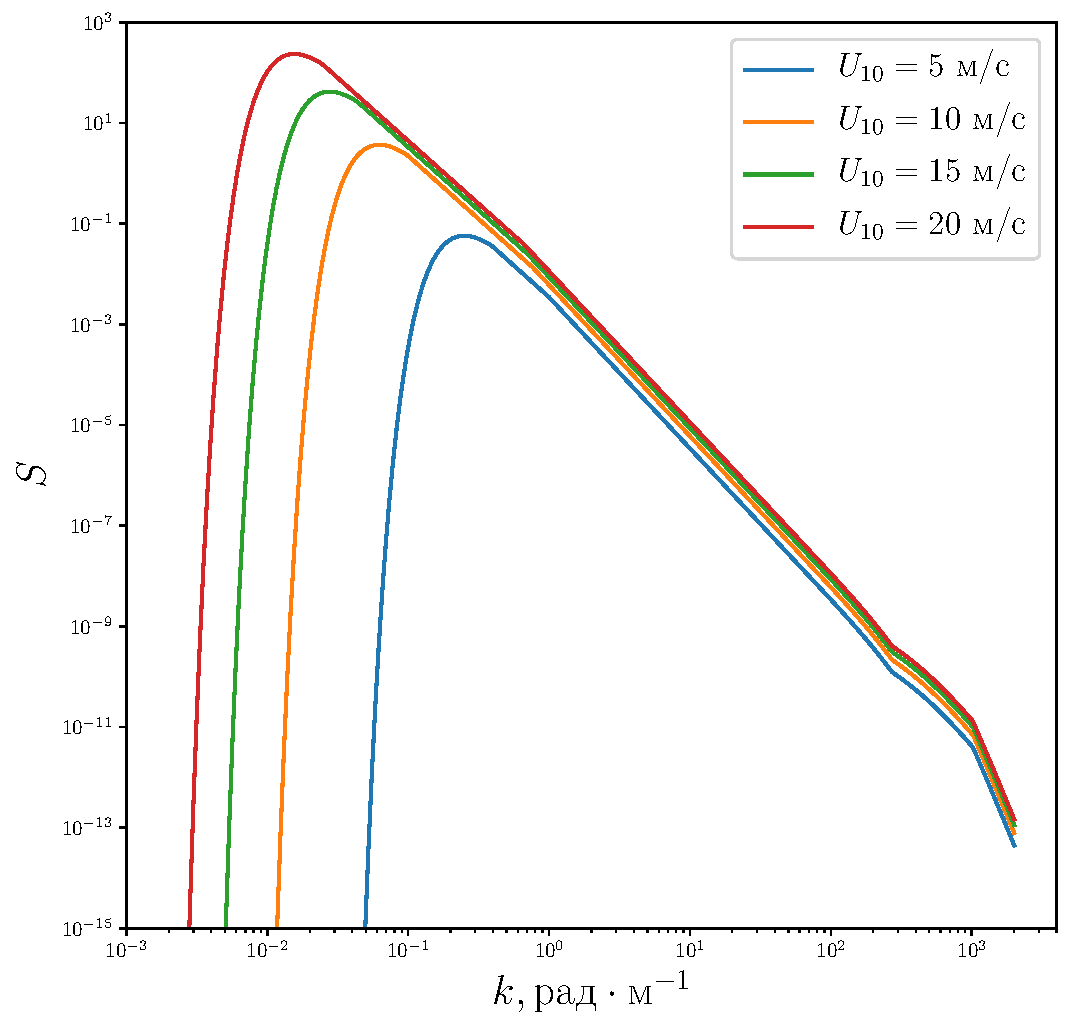
\includegraphics[width=\linewidth]{fig/full_spectrum1.pdf}
			\caption{Спектр высот $S_k(k)$ при фиксированном значении $\tilde x=20170$ и меняющейся скорости ветра}		
			\label{fig:full_spectrum1}
	\end{minipage}
	\hfill
	\begin{minipage}{0.49\linewidth}
			\centering
			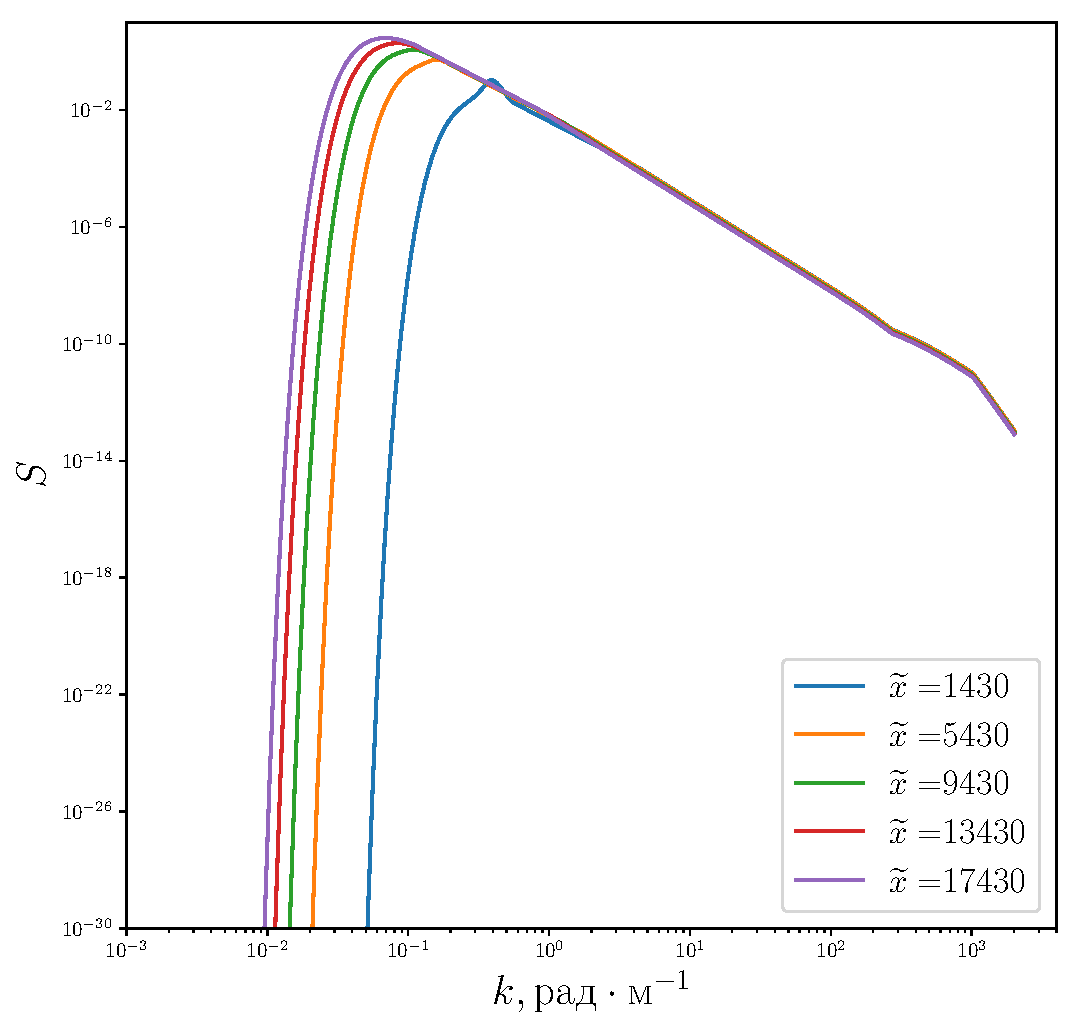
\includegraphics[width=\linewidth]{fig/full_spectrum2.pdf}
			\caption{Спектр высот $S_k(k)$ при фиксированном значении скорости ветра 
			$U=10$ м/с и меняющемся разгоне}		
			\label{fig:full_spectrum2}
	\end{minipage}
\end{figure}


\begin{figure}[h!]
	\begin{minipage}{0.49\linewidth}
			\centering
			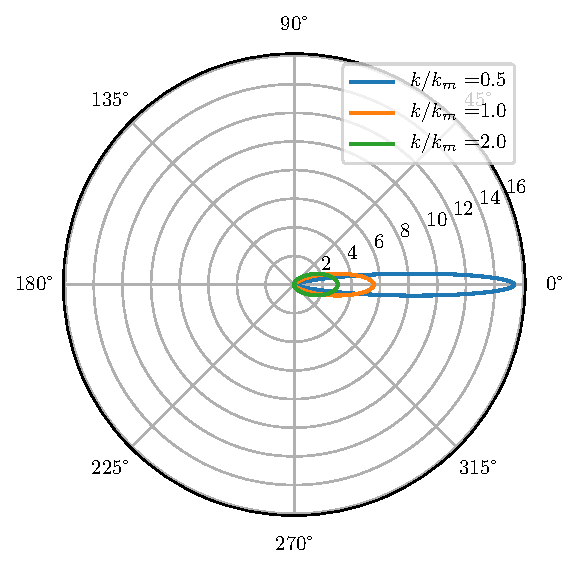
\includegraphics[width=\linewidth]{fig/full_angles1.pdf}	
	\end{minipage}
	\hfill
	\begin{minipage}{0.49\linewidth}
			\centering
			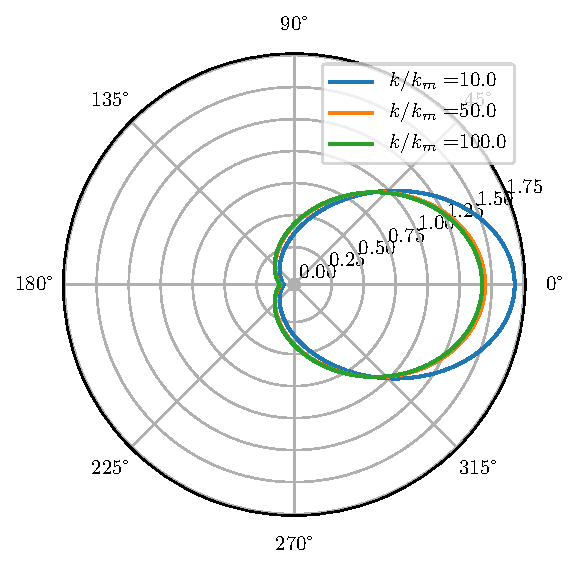
\includegraphics[width=\linewidth]{fig/full_angles2.pdf}
	\end{minipage}
	\caption{Угловое распределение $\Phi_k(\phi)$ в полярных координатах для разных соотношений $k/k_m$, где $k_m$- координата пика $S_k(k)$ при фиксированной скорости ветра}
	\label{fig:full_angles}
\end{figure}


Графики $S_k(k)$ и $\Phi_k(k)$ для наглядности изображены на рис.\ref{fig:full_spectrum1}-\ref{fig:full_spectrum2}  и $\ref{fig:full_angles}$ соответственно. И далее $k_m $-- координата пика $S_k(k)$. Стоит заметить, что
 % число гармоник $N$, используемых для моделирования, прямо пропорционально зависит от скорости ветра. 
 с ростом скорости ветра число используемых гармоник для получения одинакового качества моделирования возрастает.
 Критерием выбора оптимального числа гармоник была выбрана близость корреляционных функций высот $M$ и наклонов $M_{\theta}$ реального и модельного полей:
\begin{gather*}
	M_{\zeta}(\rho)= \int S_k(k) \cos(k \rho)\dd{k} \\
	\tM(\rho)= \sum_{n=1}^N \frac{A^2_n}{2}\cos(k_n \rho)\\
	M_{\theta}= \int k^2 S_k(k)\cos(k \rho) \dd{k} \\
	\tM_{\theta}(\rho)=\sum_{n=1}^N \frac{A_n^2}{2} k_n^2 \cos(k_n \rho)
\end{gather*}





Вообще говоря, вместе с практическими моделями для $S_k$ и $\Phi_k$ из [\ref{model}] этого достаточно, чтобы смоделировать поверхностное волнение, но без оптимизации выбора $k_n$ и $\phi_m$ счёт достаточно качественной поверхности будет длиться  слишком долго. В данной работе вопрос выбора $\phi_m$ не рассматривается и при моделировании используется эквидистантный шаг, а вопросом выбора $k_n$ мы и зададимся далее. 


\section{Реальное и модельное поля уклонов и высот поверхностного волнения}
\begin{figure}[h!]
	\begin{minipage}{0.49\linewidth}
			\centering
			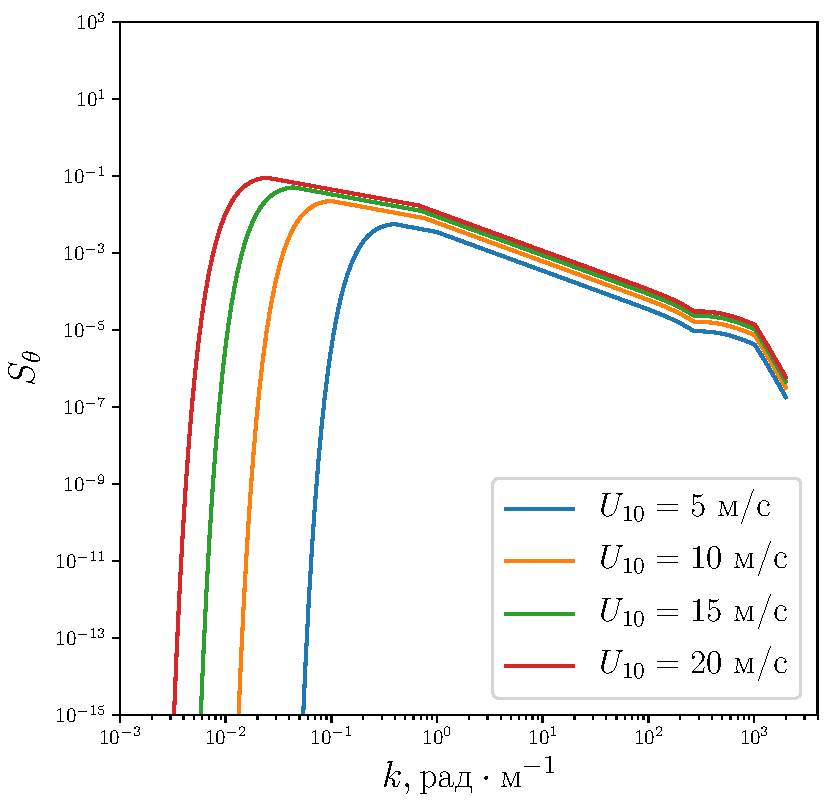
\includegraphics[width=\linewidth]{fig/full_spectrum3.pdf}
			\caption{Спектр наклонов $S_{\theta}(k)$ при фиксированном значении $\tilde x=20170$ и меняющейся скорости ветра}		
			\label{fig:full_spectrum3}
	\end{minipage}
	\hfill
	\begin{minipage}{0.49\linewidth}
			\centering
			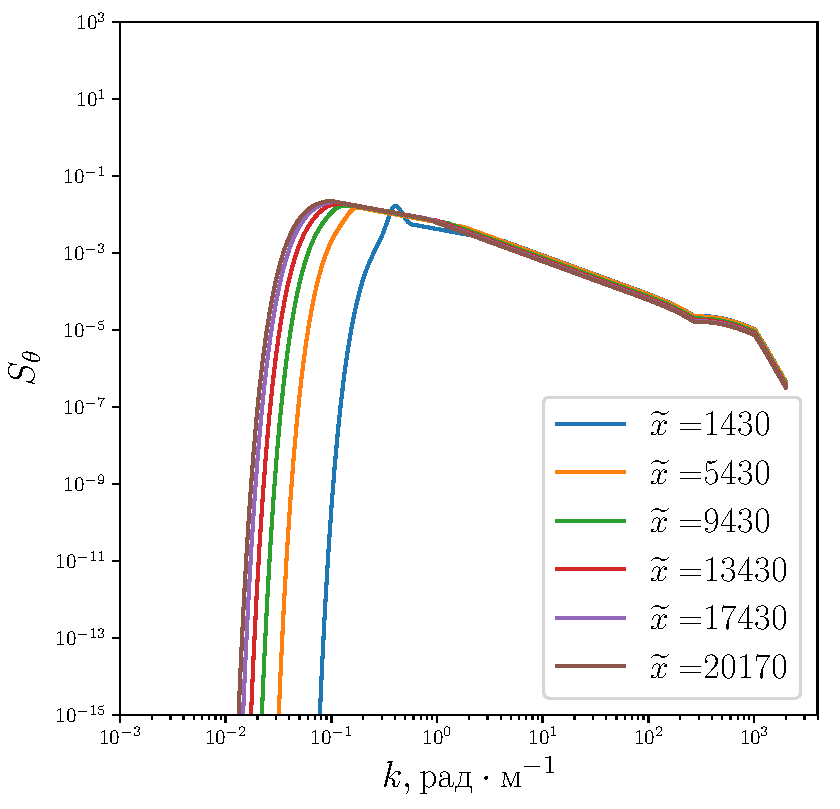
\includegraphics[width=\linewidth]{fig/full_spectrum4.pdf}
			\caption{Спектр наклонов $S_{\theta}(k)$ при фиксированном значении скорости ветра 
			$U=10$ м/с и меняющемся разгоне}		
			\label{fig:full_spectrum4}
	\end{minipage}
\end{figure}
Обратимся сначала к задаче моделирования случайного одномерного поля уклонов взволнованной поверхности. 

Пусть реальное случайное поле высот имеет корреляционную функцию 
\begin{equation}
	M=\mean {\zeta(r) \zeta(r+\rho)},
\end{equation} связанную с энергетическим спектром $S$ соотношением, следующим из \eqref{eq:3}, \eqref{eq:10} при $\Phi(\theta)=\delta(\theta)$:
\begin{equation}
	\label{eq:correlation}
	M(\rho)= \int\limits_0^{\infty} S_k(k)\cos(k \rho) \dd{k}, 
\end{equation}
Представим модельное поле высот в виде суммы N синусоид с детерминированными амплитудами $a_i$ и случайными фазами $\varphi_i$:
\begin{equation}
	\zeta(r)=\sum_{i=1}^N a_i \sin(k_ir+\varphi_i), 
\end{equation}
где фаза $\phi_i$ равномерно распределена в интервале $[0,2\pi]$. Соответствующая этому полю корреляционная функция имеет вид
\begin{equation}
	\widetilde M(\rho)=\sum\limits_{i=1}^N b_i \cos(k_i \rho),
\end{equation}

где $b_i=\frac{a_i^2}{2}$.

Энергетический спектр модельного поля уклонов представляет собой набор дельта-функций, отличных от нуля в узлах $k_i$. Огибающей спектра является кривая, проходящая через точки с абсциссами $k_i$ и ординатами $b_i$. Вопросам определения величин $b_i$ и $k_i$ 
посвящены следующие разделы работы.

Естественным способом размещения $k_i$ будет являться следующий метод:
необходимая область разбивается на $N$ участков одинаковой ширины $\Delta k$, а узлы располагаются в точках $k_i=i \Delta k, i=1,2\dots N$, т.е. эквидистантно.
Амплитуды спектральных составляющих определяются следующим соотношением:
\begin{equation}
	b_i = \int\limits_{(i-1)\Delta k}^{i \Delta k} S_k(k) \dd{k}
\end{equation}
При этом, из \eqref{eq:correlation} можно заметить, что сумма всех $b_i$ равна дисперсии реального поля
\begin{equation}
	M(0)=\sigma^2=\int\limits_0^{\infty} S_k(k) \dd{k}
\end{equation}
Однако, при таком способе моделирования корреляционная функция $\tM(\rho)$ является
периодической. Для иллюстрации на рис.\ref{fig:ca0} приведены примеры расчёта этой функции для скорости ветра $U=10 \frac{\text{м}}{\text{c}}$ и $N=256$. Конечно, период этой функции может быть удлинён, но это достигается путём увеличения гармоник.
Как видно из рис. \ref{fig:ca05} даже при неразумно большом числе гармоник период корреляционной функции недостаточно большой, что ставит под сомнение применимость такого метода моделирования.

\begin{figure}[h!]
	\begin{minipage}{0.49\linewidth}
			\centering
			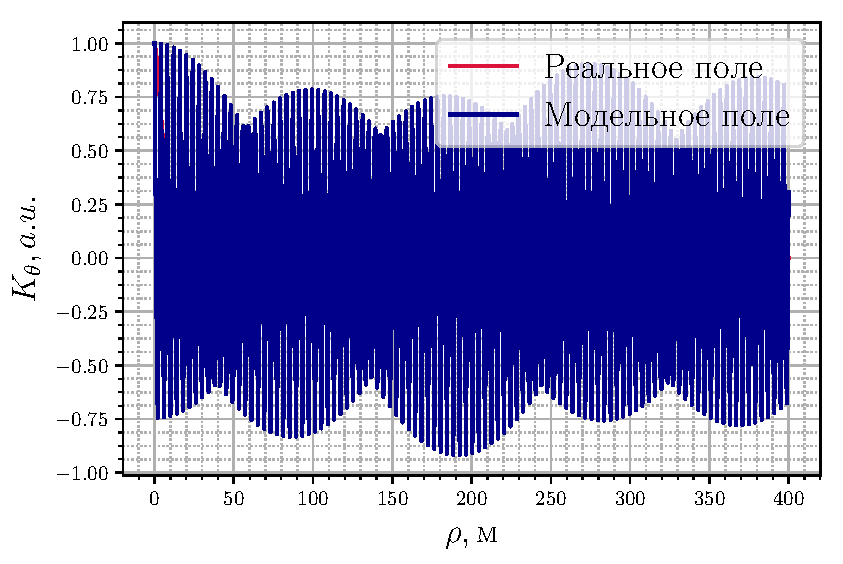
\includegraphics[width=\linewidth]{fig/correlation_height_slopes0.pdf}
			\label{fig:ch0}		
	\end{minipage}
	\hfill
	\begin{minipage}{0.49\linewidth}
			\centering
			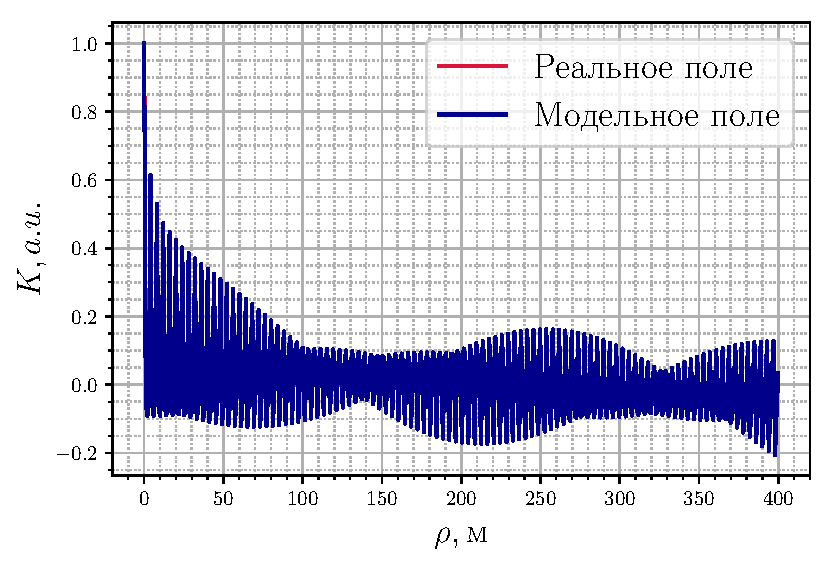
\includegraphics[width=\linewidth]{fig/correlation_angles_slopes0.pdf}
	\end{minipage}
	\caption{Корреляционные функции высот и уклонов при эквидистантном расположении узлов. $U=10 \frac{\text{м}}{c}$, $N=256$}
	\label{fig:ca0}		
\end{figure}

\begin{figure}[h!]
	\begin{minipage}{0.49\linewidth}
			\centering
			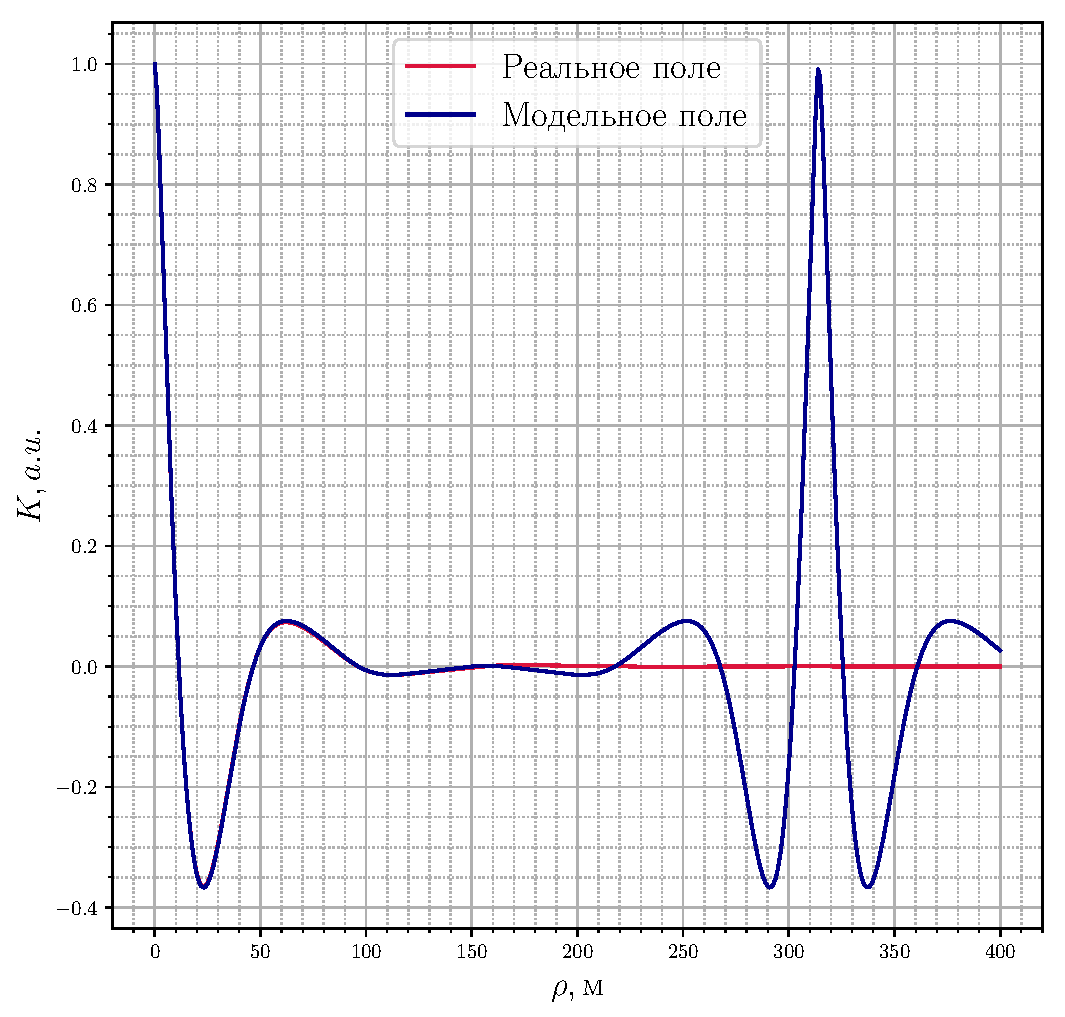
\includegraphics[width=\linewidth]{fig/correlation_height5_slopes2.pdf}
	\end{minipage}
	\hfill
	\begin{minipage}{0.49\linewidth}
			\centering
			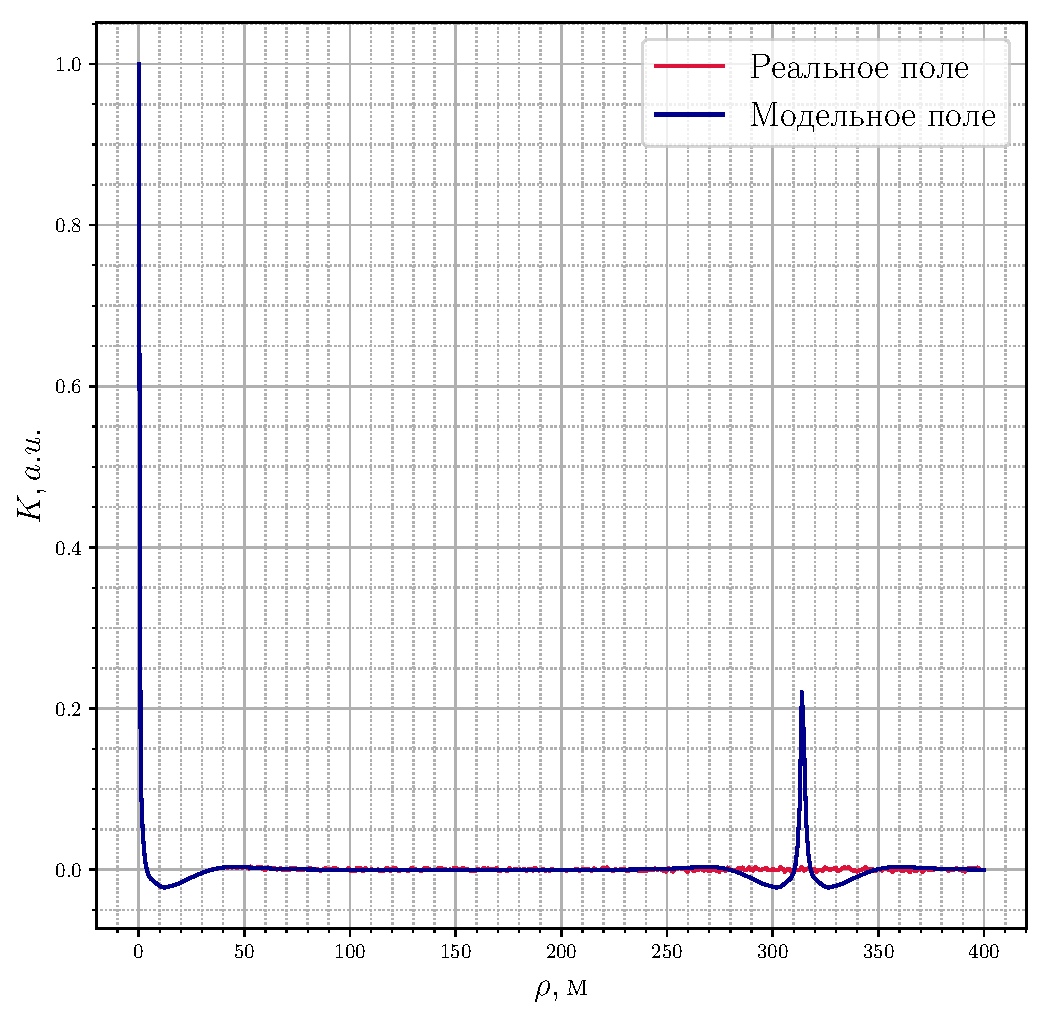
\includegraphics[width=\linewidth]{fig/correlation_angles5_slopes2.pdf}
	\end{minipage}
	\caption{Корреляционные функции высот и уклонов при эквидистантном расположении узлов. $U=10 \frac{\text{м}}{c}$, $N=10^5$}
	\label{fig:ca05}		
\end{figure}
Чтобы функция $\tM(\rho)$ не была периодической, необходимо лишь неэквидистантно расположить узлы $k_i$ на оси частот. Например, можно использовать различные детерминированные способы расположения узлов на оси частот.

Поскольку волновой спектр 
(см. рис. \ref{fig:full_spectrum1},
\ref{fig:full_spectrum3}) удобно представим в логарифмическом масштабе, то довольно естественно располагать узлы  в логарифмическом масштабе. Графики зависимости функции корреляции $\tM(\rho)$ от переменной $\rho$ изображены на рис.\ref{fig:ca1}. Очевидно, что такой способ значительно лучше, чем первый способ. Функция корреляции высот хорошо совпадает с функцией реального поля. Однако, с функцией корреляции наклонов проблем возникает больше, поскольку она быстро принимает шумовой характер. 

\begin{figure}[h!]
	\begin{minipage}{0.49\linewidth}
			\centering
			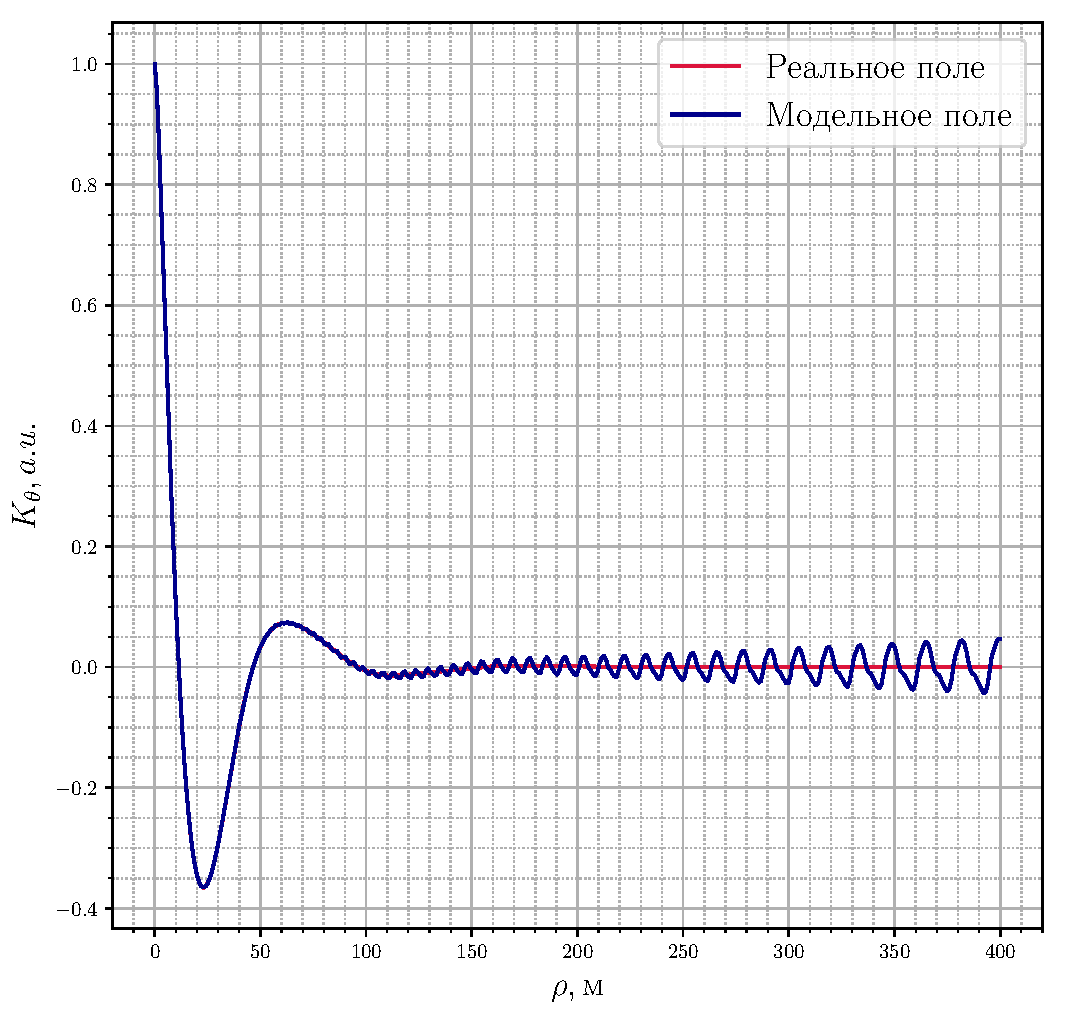
\includegraphics[width=\linewidth]{fig/correlation_height_slopes1.pdf}
			\label{fig:ch1}		
	\end{minipage}
	\hfill
	\begin{minipage}{0.49\linewidth}
			\centering
			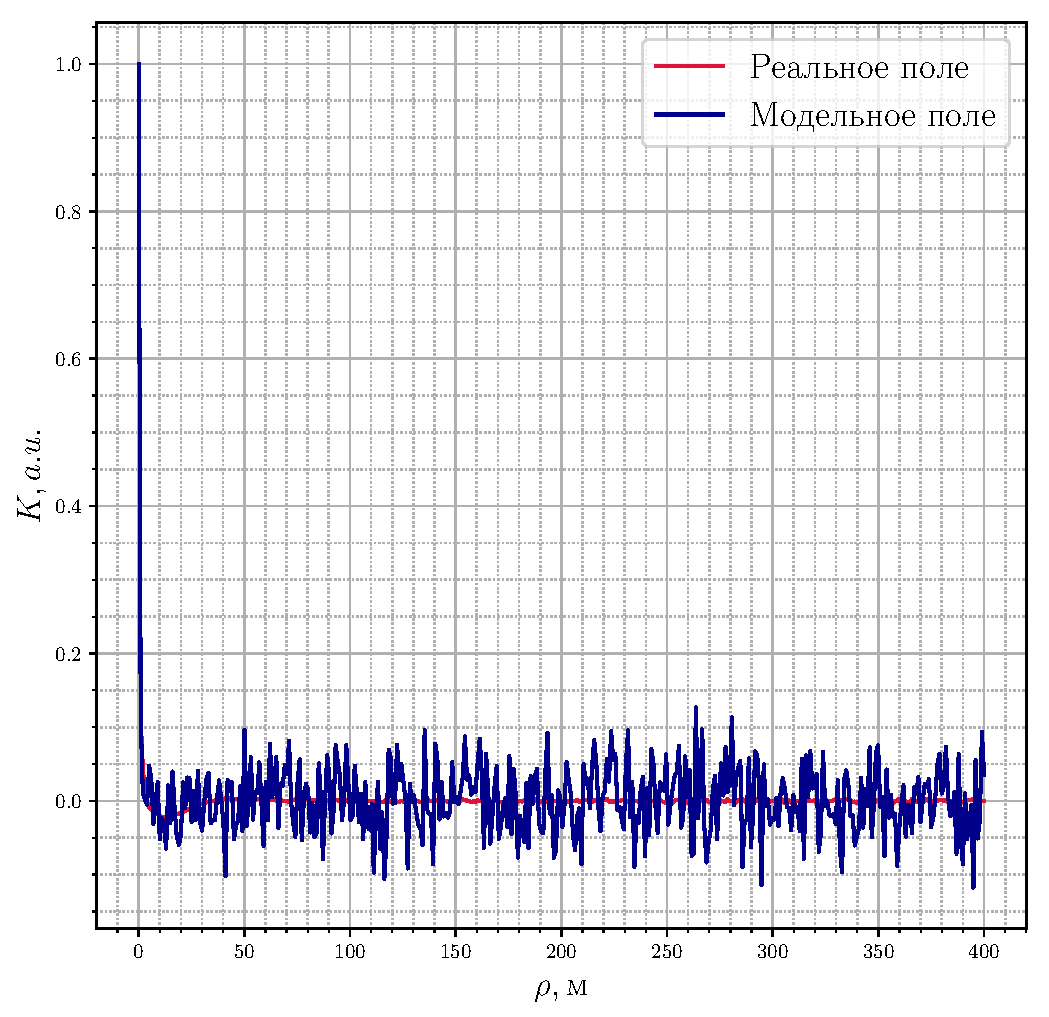
\includegraphics[width=\linewidth]{fig/correlation_angles_slopes1.pdf}
	\end{minipage}
	\caption{Корреляционные функции высот и уклонов при логарифмическом расположении узлов. $U=10 \frac{\text{м}}{c}$, $N=256$}
	\label{fig:ca1}		
\end{figure}



Способов выбора узлов по детерминированному закону существует бесконечно много, но наилучшими следует считать те способы, которые обеспечивают наименьший уровень <<шума>> на <<хвосте>> корреляционной функции $\tM(\rho)$.

\subsection{Метод <<отбеливания>> спектра}
Допустим что величины $k_i$ не находятся в дробно-рациональных отношениях друг к другу. В этом случае можно полагать, что сложение гармонических составляющих с частотами $k_i$ и амплитудами $b_i$ при больших $\rho$ происходит <<некогерентным>> образом. При этом мощность <<шума>> функции $\tM(\rho)$ определяется выражением 
$\displaystyle \sigma^2_{noise}= \sum_{i=1}^N \frac{b_i^2}{2}$. В области малых $\rho$, напротив, гармоники суммируются <<когерентно>> и соответствующая <<мощность>> равна 
$\displaystyle \tM^2(0)=\qty(\sum_{i=1}^N b_i)^2$. Образуем величину 

\begin{equation}
	\label{eq:Q}
	Q=\frac{\sigma^2_{noise}}{\tM^2(0)},
\end{equation} которая характеризует относительную мощность шумов. Минимум этой величины находится путём решения системы уравнений $\pdv{Q}{b_i}=0$, для $i=1,2,\dots,N.$
Результатом её решения является $b_1=b_2=\dots = b_N$. Спектр модельного поля при этом имеет близкий к белому вид, а выравнивание амплитуд спектральных компонент реального поля $S_k(k)$ сводится к разбиению области определения спектра $[k_{min}, k_{max}]$ на участки $\Delta k_i$, интегралы по которым от функции $S_k(k)$ имеют одно и то же значения $b_i=b_0=\sigma^2/N$.



Заметим теперь, что, рассуждая о способах разбиения интервала частот $[k_{min}, k_{max}]$ на участки $\Delta k_i$, мы оставляли нерешенным вопрос о выборе собственно узлов спектра $k_i$ внутри этих участков. Обычно узел $k_i$ ставится у правой границы ячейки $\Delta k_i$. При этом, однако, оказывается, что модельная корреляционная функция плохо согласуется с реальной корреляционной функцией в области малых $\rho$. Для достижения такого согласия следует потребовать сопряжения всех производных (от первого до $N$-го порядка) функций $\tM(\rho)$ и $M(\rho)$ при $\rho=0$. Поскольку $M'_{\rho}(\rho)=\pdv[2]{M(\rho)}{\rho}$, это условие эквивалентно требованию сопряжения моментов спектров модельного и реального полей, которое записывается в виде 
\begin{equation}
	\sum_{i=1}^N b_ik_i^{2p}=\int\limits_{0}^{\infty} k^{2p}S\dd{k},
\end{equation}
для $p=1,2,\dots,N.$

Полученная система N уравнений для N неизвестных $k_i$ не имеет общего решения и потому может анализироваться лишь численно, что тоже связано со значительными сложностями.



Наиболее простое решение вопроса о выборе узлов заключается в том, чтобы потребовать выполнения облегченного, по сравнению с предыдущим, условия сопряжения вторых моментов модельного и реального спектров высот:
\begin{equation}
	b_i k_i^2=\int\limits_{\Delta k_i} k^2 S_k(k)  \dd{k}.
\end{equation}

Из него непосредственно следует правило нахождения узлов $k_i$. В частности, получаем
\begin{equation}
	\label{eq:ki}
	k_i=\sqrt\frac{1}{b_0} \int\limits_{\Delta k_i} k^2 S \dd{k}.
\end{equation}
Правило расположения узлов \eqref{eq:ki} проиллюстрировано на рис.\ref{fig:splits}.

\begin{figure}[H]
	\begin{minipage}{0.49\linewidth}
			\centering
			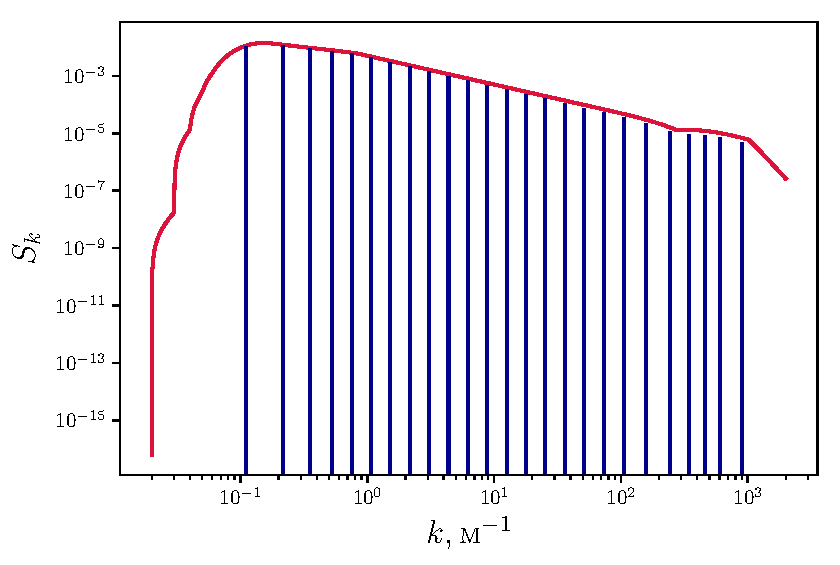
\includegraphics[width=\linewidth]{fig/split_slopes}	
	\end{minipage}
	\hfill
	\begin{minipage}{0.49\linewidth}
			\centering
			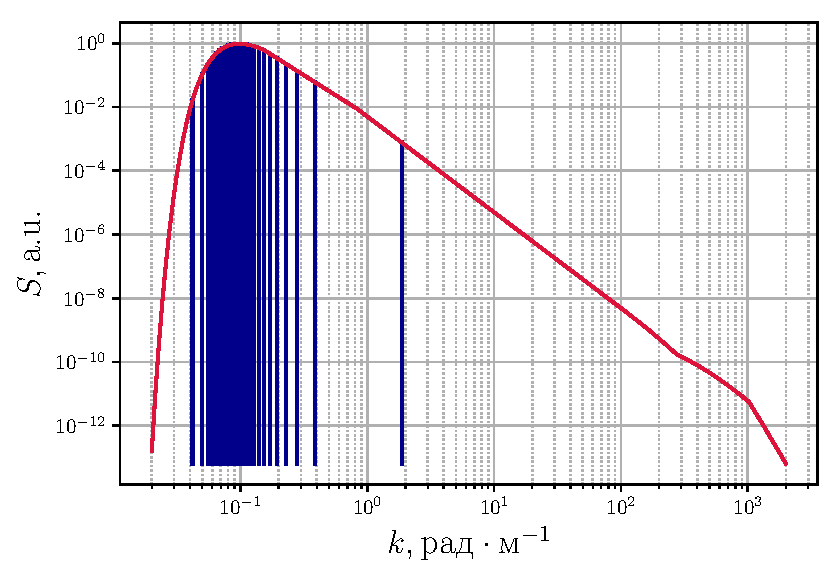
\includegraphics[width=\linewidth]{fig/split_height}
	\end{minipage}
	\caption{Расположении узлов по методу <<отбеливания>> спектра  для наклонов и высот соответственно. $U=10 \frac{\text{м}}{c}$, $N=25$}
	\label{fig:splits}		
\end{figure}


Такой способ выбора узлом, как нетрудно убедиться, обеспечивает сопряжения корреляционных функций реального и модельного полей по второй производной в нуле, или, иначе говоря, равенство дисперсий кривизн этих полей. 




Стоит сказать, что весь этот раздел был написан для поля высот $S_k(k)$, но те же рассуждения можно провести и для поля наклонов $S_{\theta}(k)$, которое связано с полем высот соотношением $S_{\theta}=k^2 S_k(k)$. Таким образом, положив 
\begin{equation}
	S_k(k)\longrightarrow k^2 S_k(k)
\end{equation}
мы можем получить уравнения для моделирования поля наклонов. 

\begin{figure}[H]
	\begin{minipage}{0.49\linewidth}
			\centering
			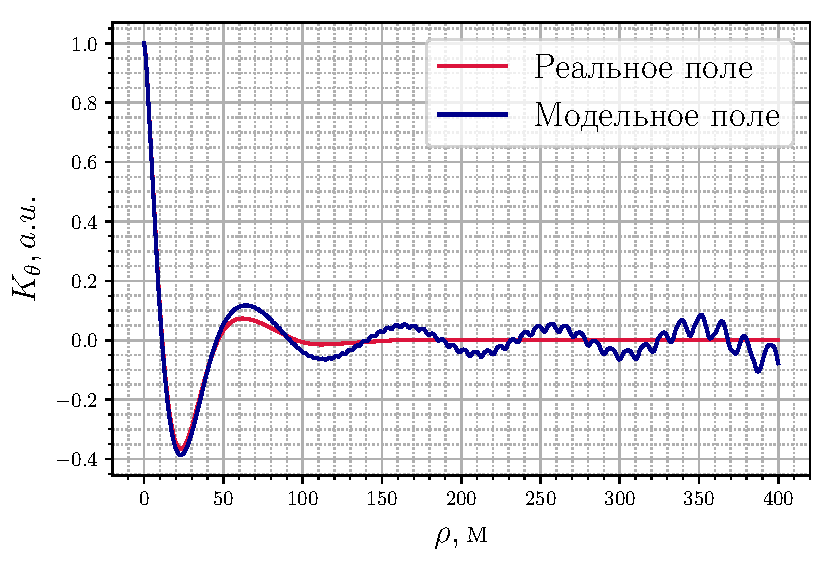
\includegraphics[width=\linewidth]{fig/correlation_height_slopes2.pdf}
			\label{fig:ch21}		
	\end{minipage}
	\hfill
	\begin{minipage}{0.49\linewidth}
			\centering
			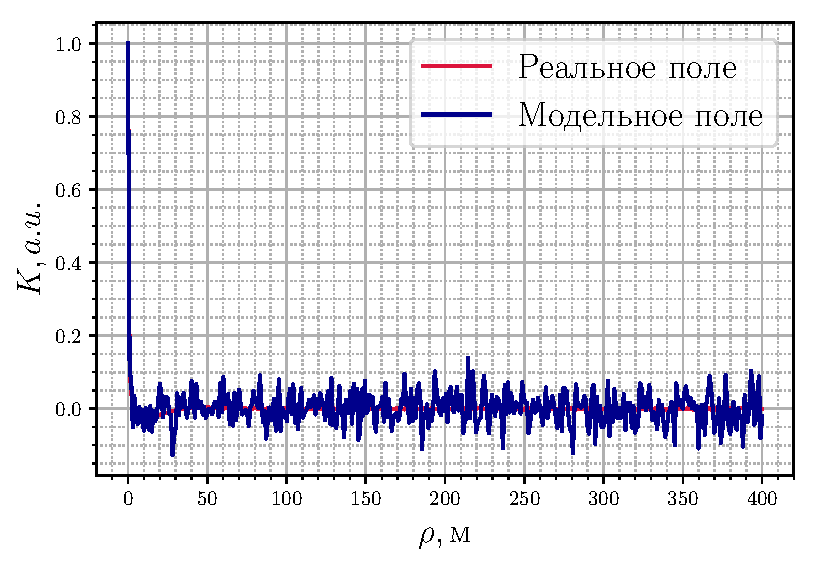
\includegraphics[width=\linewidth]{fig/correlation_angles_slopes2.pdf}
	\end{minipage}
	\caption{Корреляционные функции высот и уклонов при расположении узлов по методу <<отбеливания>> спектра для уклонов. $U=10 \frac{\text{м}}{c}$, $N=256$}
			\label{fig:ca21}		
\end{figure}


\begin{figure}[H]
	\begin{minipage}{0.49\linewidth}
			\centering
			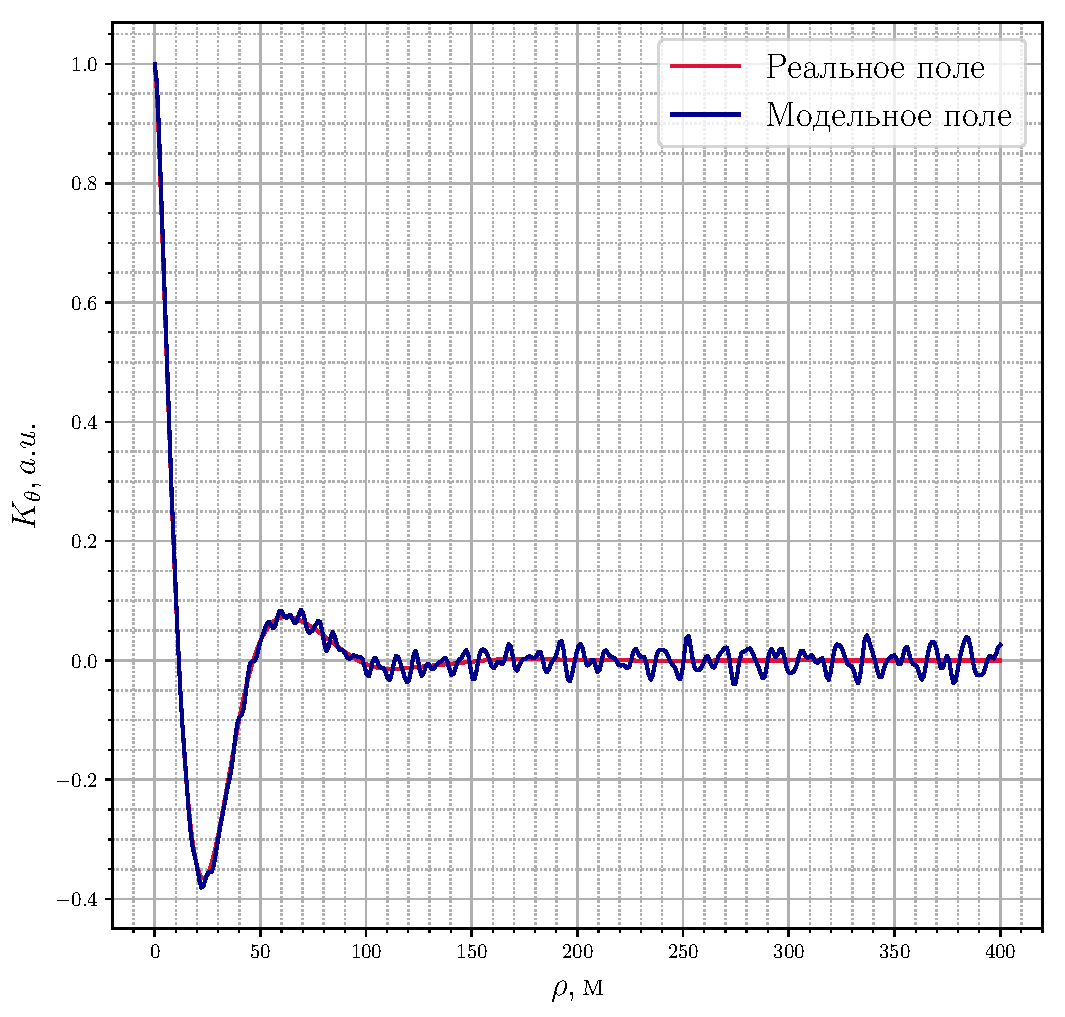
\includegraphics[width=\linewidth]{fig/correlation_height_height2.pdf}
			\label{fig:ch22}		
	\end{minipage}
	\hfill
	\begin{minipage}{0.49\linewidth}
			\centering
			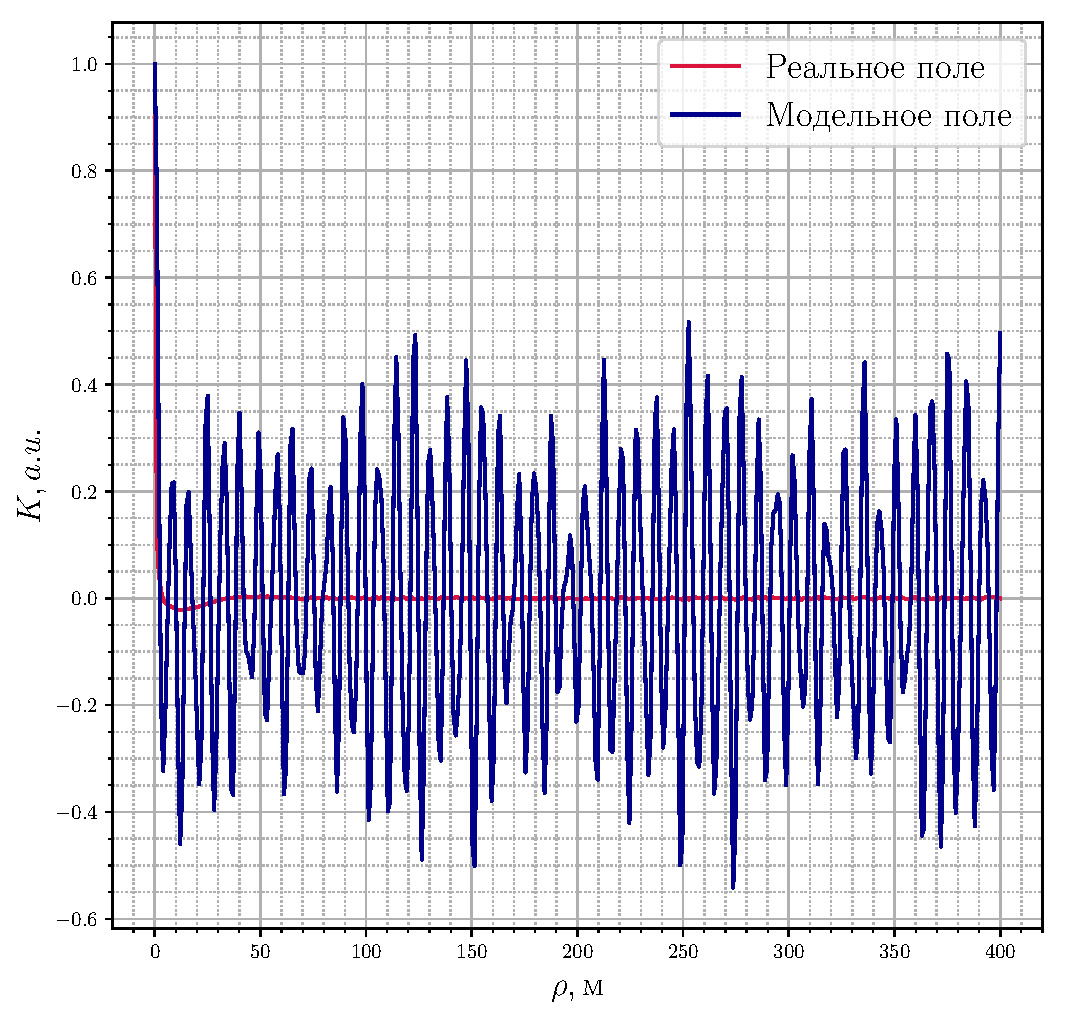
\includegraphics[width=\linewidth]{fig/correlation_angles_height2.pdf}
	\end{minipage}
	\caption{Корреляционные функции высот и уклонов при расположении узлов по методу <<отбеливания>> спектра для высот. $U=10 \frac{\text{м}}{c}$, $N=256$}
			\label{fig:ca22}		
\end{figure}
На рис. \ref{fig:ca21} и \ref{fig:ca22} построены графики зависимости корреляционных функций высот и уклонов для метода <<отбеливания>> спектра, примененного соответственно для наклонов и высот. Нетрудно заметить, что этот метод лучше предыдущих работает для одной выбранной функции и превосходит в этом логарифмическое расположение, но этот метод дает большую ошибку для другой функции корреляции. Это особенно заметно на рис. \ref{fig:ca22}: поле высот $\tM$ хорошо совпадает с реальным полем $M$, но $\tM_{\theta}$ очень далека от реальной. Исходя из этого,  без какой-либо модификации метода <<отбеливания>> его нельзя применять для моделирования одновременно уклонов и высот и разумнее использовать логарифмическое разбиение. Модификация же заключается в выборе новой относительной мощности шумов $Q$ (см. \eqref{eq:Q}) так, чтобы она удовлетворяла одновременно двум функциям корреляции, и её дальнейшая минимизация.  




\section{Заключение}

\begin{figure}[H]
\begin{minipage}[h]{0.45\linewidth}
	\centering
	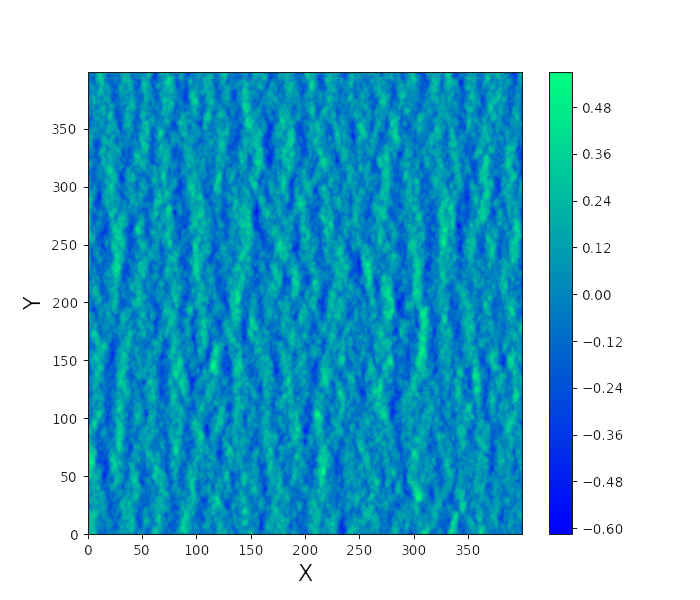
\includegraphics[width=\linewidth]{img/water5.png}
	\caption{Моделирование высот морского волнения. $N=256, ~ U_{10}=5$ }
	\label{fig:water5}
\end{minipage}
\hfill
\begin{minipage}[h]{0.45\linewidth}
	\centering
	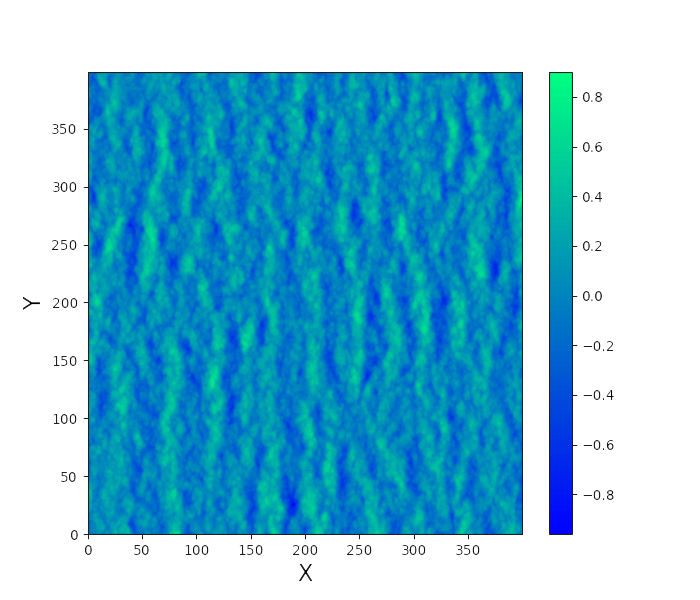
\includegraphics[width=\linewidth]{img/water6.png}
	\caption{Моделирование высот морского волнения. $N=256, ~ U_{10}=6$ }
	\label{fig:water6}
\end{minipage}

\vfill
\begin{minipage}[h]{0.45\linewidth}
	\centering
	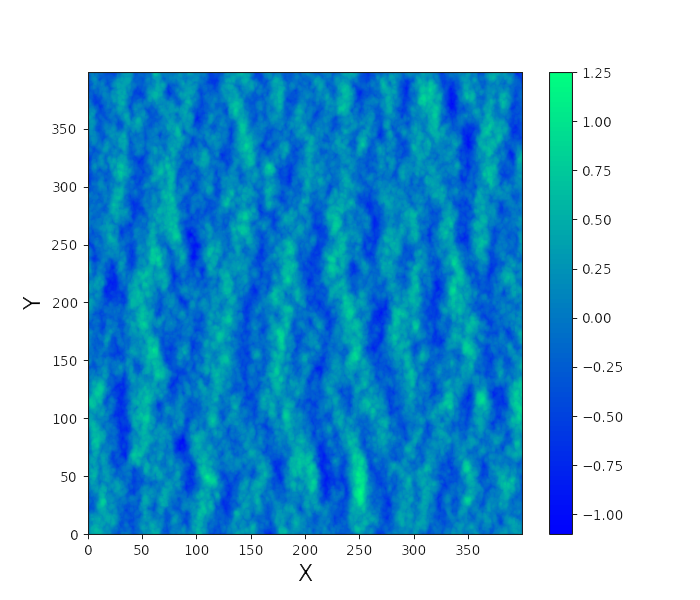
\includegraphics[width=\linewidth]{img/water7.png}
	\caption{Моделирование высот морского волнения. $N=256, ~ U_{10}=7$  }
	\label{fig:water7}
\end{minipage}
\hfill
\begin{minipage}[h]{0.45\linewidth}
	\centering
	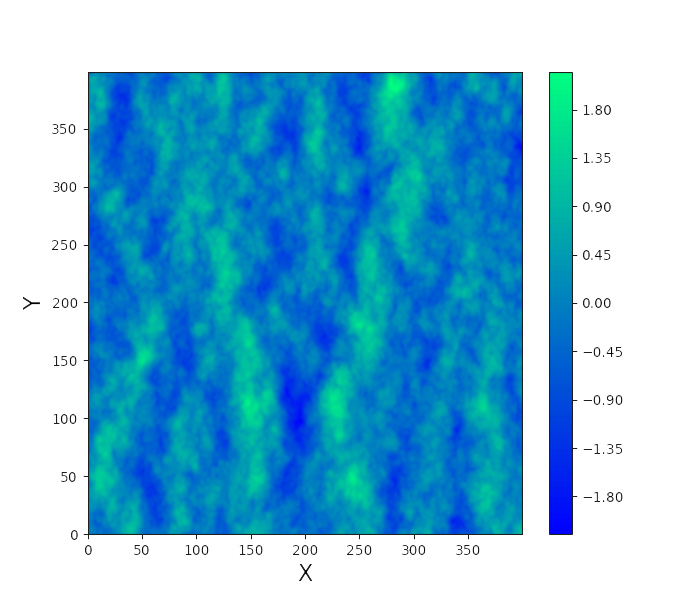
\includegraphics[width=\linewidth]{img/water10.png}
	\caption{Моделирование высот морского волнения. $N=256, ~ U_{10}=10$ }
	\label{fig:water10}
\end{minipage}
\end{figure}

В задаче о рассеянии электромагнитного СВЧ-поля взволнованной водной поверхностью всё ещё остается много вопросов. В то же время радиолокаторы широко применяются для решения самых разнообразных прикладных задач, например, измерения скорости и направления приповерхностного ветра, высоты значительного волнения, скорости течений и температуры воды. Алгоритмы, которые применяются для обработки данных, далеко не всегда позволяют получить информацию о состоянии приповерхностного слоя с необходимой точностью, а кроме того, существующие задачи радиолокаторы могут измерять далеко не все характеристики поверхности, представляющие интерес.

Обе эти задачи можно решить с помощью численного моделирования. В данной работе рассмотрен метод моделирования поверхности суммой синусоидальных составляющих с детерминированными амплитудами и случайными фазами. Выбор частот осуществлялся несколькими способами их расположения на частотной оси. 
Было рассмотрено эквидистантное, логарифмическое и детерминированное  распределение гармоник, сделаны выводы о их практической применимости и точности расчётов.

В детерминированном способе частоты располагались внутри участков, имеющих одно и то де постоянное значение интеграла от спектра волнения. Этот метод -- метод <<отбеливания>> спектра -- является новым и требует модификации, т.к. в его текущем виде можно <<отбелить>> лишь один спектр высот или наклонов (см. рис.\ref{fig:ca22}, \ref{fig:ca21}). В дальнейшем планируется выбором некой новой величины $Q$ (см.\eqref{eq:Q}) добиться одновременного <<отбеливания>> спектра для наклонов и высот морского волнения. Пока это не осуществленно, оптимальным стоит считать логарифмический метод расположения, который уступает методу <<отбеливания>> для одиночно взятого спектра, но обеспечивает б\'{о}льшую точность при одновременном моделировании высот и наклонов. 



На рисунках \ref{fig:water5}-\ref{fig:water10} представлены 
смоделированные  поля высот для разных скоростей ветра.

% \footnote
{Модель написала на языке Python v3.7 с использованием библиотек NumPy и SciPy, отчёт по практике и презентация к ней оформлены в издательской системе \LaTeX. Актуальную версию программы можно найти на 
Github.
\vfill
\begin{center}
\qrcode{https://github.com/KirillPonur/water}
\end{center}}

% В дальнейшем планируется усовершенствовать выбор азимутальных координат $\phi$, а также выбором некой новой величины $Q$ (см.\eqref{eq:Q}) добиться одновременного <<отбеливания>> спектра для наклонов и высот морского волнения.
% 


\appendix
\section{Приложение}
\label{model}
\subsection{Модель спектра волнения}

Для моделирования волнения используется следующая модель спектра волнения, предложенного в \cite{Karaev2}: 
\begin{equation}
	\label{eq:Sw}
	\begin{cases}
		S(\omega)=S_J(\omega), &  0<\omega\leq 1.2\,\omega_m\\
		S(\omega)= \frac{\alpha_2}{\omega^4}, &  1.2 \,\omega_m < \omega \leq \alpha_m \omega_m\\
		S(\omega)= \frac{\alpha_3}{\omega^5}, &   \alpha_m \omega_m< \omega \leq \omega_gk\\
		S(\omega)= \frac{\alpha_4}{\omega^{2.7}}, & \omega_{gk}<\omega\leq \omega_h\\
		S(\omega)= \frac{\alpha_5}{\omega^5}, & \omega_h<\omega,
	\end{cases}
\end{equation}
где коэффициенты $\alpha_i$ задаются следующим образом:
\begin{equation}
	\label{eq:alpha_i}
	\begin{cases}
		\alpha_2=S_J(1.2 \omega_m)\cdot (1.2 \omega_m)^4 \\
		\alpha_3=a_2\cdot \alpha_m \omega_m \\
		\alpha_4= \frac{\alpha_3}{\omega^{2.3}_{gk}} \\
		\alpha_5 = \alpha_4 \cdot \omega_h^{2.3} \\
		\alpha_m = f(U_{10}), & 
	\end{cases}
\end{equation}
$U_{10} \text{-- скорость ветра на высоте 10 метров над уровнем моря,}$ а $S_J(\omega)$-- спектр JONSWAP:
\begin{equation}
\label{eq:Sj}
	S_J(\omega)\sim \frac{g^2}{\omega^{5}}\exp{-\qty(\frac{\omega_m}{\omega})^4}
	\cdot \gamma^{\exp{-\omega^2}}
\end{equation}
Стоит отметить, что в конечном счете формулы \eqref{eq:Sw},\eqref{eq:alpha_i},\eqref{eq:Sj} в модели использовались в $k-$представлении, т.е.  был выполнен переход $S(\omega)\rightarrow S_k(k)$


\subsection{Модель углового распределения}
Угловое распределение $\Phi_{\omega}$ в данной работе описывается следующей формулой:
\begin{equation}
	\Phi_{k} (k, \phi)= A\cdot \cosh^{-1}\{2B(k) \phi\}, ~~ -\pi\leq \phi \leq \pi,
\end{equation}
где $\phi=\phi_m = \phi_w$, $\phi_w$-- генеральное направление распространения волнения,
$\phi_m$-- текущий азимутальный угол, $A$-- нормировочный коэффициент.




Дисперсионное уравнение в данной работе имеет вид:
\begin{equation}
	\label{eq:w_k}
	\omega(k)=\sqrt{gk+a\cdot k^3},
\end{equation}
% Значения и физический смысл всех коэффициентов можно найти в \cite{Karaev1}, а также в исходном коде программы 
% (\href{https://github.com/KirillPonur/water}{github.com/KirillPonur/water})

\newpage
\begin{thebibliography}{}
	\bibitem{Rytov} \textit{С.М. Рытов}, Введение в статистическую радиофизику // Изд. 2-е, перераб. и доп. - Москва : Наука, 1976. - Ч. 1. Случайные процессы \S\S 14-18, 38-42 
	\bibitem{Karaev1} \textit{В.Ю.Караев, М.Б. Каневский, Г.Н. Баландина}, Численное моделирование поверхностного волнения и дистанционное зондирование // Препринт №552 ИПФ РАН, 2002, С.1-10.
	\bibitem{Veber} \textit{В.Л. Вебер}, О моделировании случайного профиля морской поверхности // Изв. вузов. Радиофизика. 2017. Т. 60, № 4. С. 346.
	\bibitem{Karaev2} \textit{В.Ю.Караев, Г.Н. Баландина} Модифицированный спектр волнения и дистанционное зондирование // Исследование Земли из космоса, 2000, N5, C.1-12.
	\bibitem{Longe} \textit{М.С. Лонге-Хиггинс} Статистический анализ случайной движущейся поверхности // в кн.: Ветровые волны, М.: Иностранная наука, 1962, С.112-230
\end{thebibliography}
\newpage
\end{document}